\documentclass{classe-tex3R}
\usepackage{style-tex3R}
\usepackage{dirtree}
\parametrage



\colorlet{colorBasic}{SlateGrey}
\colorlet{colorBracket}{DarkViolet}
\colorlet{colorKeyword}{DarkBlue}
\colorlet{colorEnvironment}{LightSeaGreen}
\colorlet{colorComment}{Green}
\colorlet{colorString}{Chocolate}
\colorlet{colorChange}{Red}
\colorlet{colorMath}{Teal}
\colorlet{colorVariable}{LightSkyBlue}
\colorlet{colorVariableDeux}{Teal}
\colorlet{colorBoolean}{Indigo}
\colorlet{colorFunction}{DarkGoldenrod}
\colorlet{colorIdentifier}{MediumOrchid}

\newcommand{\nocontentsline}[3]{}
\newcommand{\tocless}[2]{\bgroup\let\addcontentsline=\nocontentsline#1{#2}\egroup}

\lstset{
  %Réglages généraux
  backgroundcolor=\color{gray!20!white},
  basicstyle=\ttfamily\small\color{colorBasic},
  columns=fullflexible,
  aboveskip=\baselineskip,
  belowskip=0pt,
  breaklines=true,
  %Keywords
  emph={[1]
    documentclass,
    usepackage,
    definirchapitre,
    definirniveau,
    parametrage,
    bareme,
    competence,
    difficulte,
    source,
    theme,
    montitre,
    tailletexte,
    partie,
    souspartie,
    chapitre,
    visiblecmd,
    saut,
    lignes,
    ifdiapo,
    iffiche,
    ifheader,
    ifprint,
    ifactivite,
    ifbasique,
    ifbilan,
    ifcorrige,
    ifcours,
    ifTD,
    ifflash,
    ifDM,
    ifDS,
    ifinterro,
    ifcorrection,
    ifenonce,
    ifvisible,
    ifbareme,
    ifdifficulte,
    ifcompetence,
    ifsource,
    iftheme,
    ifstretch,
    ifsubfile,
    else,
    fi,
    newcounter,
    setcounter,
    stepcounter,
    thecompteurexercice,
  }, 
  emphstyle={[1]\color{colorKeyword}},
  %Environnements
  emph={[2]
    environnement,
    luacode,
    fiche,
    document,
  }, 
  emphstyle={[2]\color{colorEnvironment}},
  %Variable lua
  emph={[3]
  Type,
  Impression,
  Header,
  Taille,
  Stretch,
  Correction,
  Enonce,
  Visible,
  Competence,
  Bareme,
  Difficulte,
  Source,
  Theme,
  arg,
  str,
  },
  emphstyle={[3]\color{colorVariable}},
  %Booléens lua
  emph={[4]
  true,
  false,
  nil,
  local
  },
  emphstyle={[4]\color{colorBoolean}},
  %Fonctions lua
  emph={[5]
  mesParametres,
  NiveauUtilisateur,
  NiveauDocument,
  },
  emphstyle={[5]\color{colorFunction}},
  %Variables lua
  emph={[6]
  PAGE,
  POLICE,
  COULEURS,
  LOGOS,
  STYLESTITRES,
  TITRES,
  ENVIRONNEMENTS,
  },
  emphstyle={[6]\color{colorVariable}},
  %Variables deux lua
  emph={[7]
  enumi,
  enumii,
  itemi,
  itemii,
  sectionname,
  subsectionname,
  subsubsectionname,
  sectionnumber,
  subsectionnumber,
  subsubsectionnumber,
  sectionsformat,
  chapitrenormalformat,
  chapitreetoileformat,
  partformat,
  width,
  height,
  parindent,
  parskip,
  headertop,
  headerbottom,
  headerright,
  headerleft,
  headermarginparsep,
  headermarginparwidth,
  headerheadheight,
  headerheadsep,
  headerfootskip,
  top,
  bottom,
  right,
  left,
  marginparsep,
  marginparwidth,
  headheight,
  headsep,
  footskip,
  application,
  convention,
  definition,
  exemple,
  methode,
  propriete,
  preuve,
  remarque,
  enonce,
  correction,
  visible,
  taillefiche,
  taillediapo,
  texte,
  math,
  mathcal,
  important,
  ligne,
  interligne,
  section,
  subsection,
  subsubsection,
  carreau,
  surlignelignea,
  surligneligneb,
  boitecours,
  background,
  exercice,
  surligne,
  surlignevisible,
  rouge,
  vert,
  bleu,
  activite,
  basique,
  bilan,
  corrige,
  cours,
  DM,
  DS,
  flash,
  interro,
  TD,
  tocexercice,
  tocenonce,
  toccorrection,
  formatcours,
  tocactivite,
  tocbasique,
  tocbilan,
  toccorrige,
  toccours,
  tocDM,
  tocDS,
  tocflash,
  tocinterro,
  tocTD,
  format,
  espacement,
  titre,
  stylesections,
  },
  emphstyle={[7]\color{colorVariableDeux}},
  %Variables lua
  emph={[8]
  begin,
  end,
  if,
  elseif,
  function,
  then,
  },
  emphstyle={[8]\color{colorIdentifier}},
  %Literate
  literate={
    % {\{}{{\textcolor{colorBracket}{\{}}}1
    % {\}}{{\textcolor{colorBracket}{\}}}}1
    % {[}{{\textcolor{colorBracket}{[}}}1
    % {]}{{\textcolor{colorBracket}{]}}}1
    % {[[}{{\textcolor{colorString}{[[ }}}1
    % {]]}{{\textcolor{colorString}{]]}}}1
    % {\\}{{\textcolor{colorKeyword}{\textbackslash}}}1
    % {0}{{$\cancel{0}$}}1
    },
  %Comment
  comment=[l]{--},
  morecomment=[l]{\%},
  commentstyle=\color{colorComment},
  %Delimiters
  moredelim=[is][\color{colorChange}]{@}{@},
  moredelim=[s][\color{colorMath}]{\$}{\$},
  moredelim=[is][\color{colorString}]{||}{||},
  moredelim=[s][\color{colorString}]{[[}{]]},
  moredelim=[s][\color{colorString}]{'}{'},
  moredelim=[is][\color{colorBasic}]{//}{//},
  moredelim=[is][\color{colorComment}]{/*}{/*},
  }

\title{\bfseries style-tex3R\par}
\author{Vincent Crombez \& Frédéric Léothaud}
\date{}

\cfoot{\pagemark}
\setlength{\parskip}{\baselineskip}
\setcounter{tocdepth}{3}
\renewcommand{\sectionformat}{\LARGE\textbf{\thesection~}}
  \setkomafont{section}{\normalfont\LARGE\color{Black}\bfseries}
\renewcommand{\subsectionformat}{\Large\textbf{\thesubsection~}}
  \setkomafont{subsection}{\normalfont\Large\color{Black}\bfseries}
\renewcommand{\subsubsectionformat}{\large\textbf{\thesubsubsection~}}
  \setkomafont{subsubsection}{\normalfont\large\color{Black}\bfseries}


\begin{document}

\maketitle

\newpage

\tableofcontents

\newpage

\phantomsection
\addcontentsline{toc}{section}{Introduction}
\section*{Introduction}

La \texttt{style-tex3R} fait partie d'un projet comprenant :
%
\begin{itemize}
  \item \href{https://github.com/Tex3rivieres/TeX3R-ClasseStyle}{Une classe, un style et des templates de documents pratiques}
  \item \href{https://github.com/Tex3rivieres/TeX3R-Portable}{Un environnement LaTeX portable}
  \item \href{https://github.com/Tex3rivieres/TeX3R-Workshop}{Une extension (basée sur \texttt{latex-workshop})}
\end{itemize}

Il est préférable d'aller d'abord lire la documentation de \texttt{classe-tex3R} qui explique l'ensemble des commandes disponibles. 

L'objectif de ce guide est de guider la personnalisation du style à appliquer aux environnements et commandes de la \texttt{classe-tex3R}, afin d'avoir une apparence propre selon les goûts de chacun, tout en gardant la possibilité de transférer son document à un autre utilisateur de la \texttt{classe-tex3R}, qui lui le compilera avec le style de son choix.

\newpage

\section{Créer un nouveau style}

Afin d'utiliser son style personnalisé, il suffit de créer une copie du fichier \texttt{style-tex3R.sty} dans le même dossier, de le renommer \texttt{monstyle.sty} et de travailler sur ce dernier. Le fichier \texttt{style-tex3R} se trouve dans l'emplacement suivant :

\saut{ligne} %#1=fiche/diapo

\dirtree{%
.1 TeX3R-ClasseStyle.
  .2 documentation.
  .2 templates.
  .2 tex.
    .3 fonts.
    .3 lualatex.
      .4 tex3R.
        .5 {classe-tex3R.cls}.
        .5 {style-tex3R.sty}.
.2 {.gitignore}.
.2 {README.md}.
}

Une fois le fichier \texttt{monstyle.sty} créé il est nécessaire d'ouvrir MiKTeX Console et de faire Tasks > Refresh file name database.

Ensuite, pour appeler \texttt{monstyle} dans un nouveau document, il suffit de changer le préambule comme suit :

\begin{lstlisting}
\documentclass{classe-tex3R}
\usepackage{monstyle}
\parametrage

\begin{document}

%Le texte du document

\end{document}
\end{lstlisting}

\section{Principe de modification}

\texttt{classe-tex3R} et \texttt{style-tex3R} sont codés majoritairement en \texttt{lua}. L'idée derrière cela est d'avoir une part minimale de choses à modifier dans le style, dans des chaînes de caractères \texttt{lua}, qui seront ensuite insérées et utilisées par les commandes de la classe. Ceci étant, les choses pouvant être modifiées sont toujours entre \texttt{[[ ]]} ou entre \texttt{' '} qui sont les délimiteurs des chaînes de caractères en \texttt{lua}. 

Cette expérience simplifiée évite d'avoir à aller voir dans de nombreuses documentations pour connaître la syntaxe exacte pour chaque paramètre. 

Par la suite, nous détaillerons chacune des fonctions \texttt{lua}, et à quoi correspondent les différentes parties modifiables.

\section{FormatUtilisateur()}

\subsection{Listes et énumérations}

\begin{lstlisting}
PAGE.enumi = ||[[ \textbf{\arabic*.~} ]]||
PAGE.enumii = [[ \textbf{\alph*.~} ]]
PAGE.itemi = [[ \textbullet ]]
PAGE.itemii = [[ $\circ$ ]]
\end{lstlisting}

\begin{itemize}
  \item \texttt{enumi} : liste numérotée de niveau 1.
  \item \texttt{enumii} : liste numérotée de niveau 2.
\end{itemize}

\texttt{\textbackslash Alph*}, \texttt{\textbackslash alph*}, \texttt{\textbackslash roman*}, \texttt{\textbackslash Roman*}, \texttt{\textbackslash arabic*}

\begin{itemize}
  \item \texttt{itemi} : liste à puces de niveau 1.
  \item \texttt{itemii} : liste à puces de niveau 2.
\end{itemize}

Possibilité de mettre n'importe quel symbole.

\subsection{Chapitre, partie et sous-partie}

\begin{lstlisting}
PAGE.sectionname = [[ \LARGE\bfseries\textcolor{couleursection} ]]
PAGE.subsectionname = [[ \Large\bfseries\textcolor{couleursubsection} ]]
PAGE.subsubsectionname = [[ \normalfont\large\bfseries\textcolor{couleursubsubsection} ]]
\end{lstlisting}

Format du texte des \texttt{\textbackslash section}, \texttt{\textbackslash subsection} et \texttt{\textbackslash subsubsection}. Pour rappel, les \texttt{\textbackslash section} ne sont pas utilisées car remplacées par les titres. Les \texttt{\textbackslash subsection} et \texttt{\textbackslash subsubsection} correspondent aux commandes \texttt{\textbackslash partie} et \texttt{\textbackslash souspartie}
 
\begin{lstlisting}
PAGE.stylesections = [[ \colorbox{#1}{\textcolor{white}{\normalfont#2\textbf{{#3}}}} ]]

PAGE.sectionnumber = [[ \stylesections{couleursection}{\LARGE}{~\Roman{section}~}\, ]]
PAGE.subsectionnumber = [[ \stylesections{couleursubsection}{\LARGE}{\Alph{subsection}}\, ]]
PAGE.subsubsectionnumber = [[ \stylesections{couleursubsubsection}{\LARGE}{\arabic{subsubsection}}\, ]]
\end{lstlisting}

\begin{itemize}
  \item \texttt{stylesections} : style du numéro devant les sections, subsections et subsubsections (par défaut un carré de couleur avec le nombre ou la lettre en blanc). Trois argument :
    \begin{itemize}
      \item \#1 = couleur
      \item \#2 = Taille du texte
      \item \#3 = Style de la numérotation (Roman, arabic, etc)
    \end{itemize}
  \item \texttt{sectionnumber} : style du numéro des \texttt{\textbackslash section}
  \item \texttt{subsectionnumber} : style du numéro des \texttt{\textbackslash subsection}
  \item \texttt{subsubsectionnumber} : style du numéro des \texttt{\textbackslash subsubsection}
\end{itemize}


\begin{lstlisting}
PAGE.sectionsformat = [[ #3 \underLine{#4}\par\vspace{0.5em} ]]
\end{lstlisting}

\texttt{sectionsformat} : formatage global des \texttt{\textbackslash section}, \texttt{\textbackslash subsection} et \texttt{\textbackslash subsubsection}. Par défaut, texte souligné sans espacement horizontal.
  \begin{itemize}
    \item \#3 = emplacement de la numérotation
    \item \#4 = emplacement du texte
  \end{itemize}

\begin{lstlisting}
PAGE.chapitrenormalformat = [[ \huge\bfseries Chapitre \thepart ]]
PAGE.chapitreetoileformat = [[]]
PAGE.partformat = [[
  \newpage
  \hfill
  \vfill
  \begin{tcolorbox}[
    colframe = black, 
    colback=white,
    coltitle=white,
    sharp corners,
    valign=center,
    top=2cm,
    bottom=2cm,
    left=0.5cm,
    enhanced,
    before skip=0cm,
  ]
  \formatchapitre
  \tcblower
  {\huge\bfseries #3}
  \end{tcolorbox}
  \hfill
  \vfill
]]
\end{lstlisting}

\begin{itemize}
  \item \texttt{chapitrenormalformat} : contenu de \texttt{\textbackslash formatchapitre} pour la commande \texttt{\textbackslash chapitre}
  \item \texttt{chapitreetoileformat} : contenu de \texttt{\textbackslash formatchapitre} pour la commande \texttt{\textbackslash chapitre*}
  \item \texttt{partformat} : formatage de la \texttt{\textbackslash part}, ce qui formate également la commande \texttt{\textbackslash chapitre}
\end{itemize}

Rappel : la commande \texttt{\textbackslash chapitre} ne sert que pour les méga-documents, page de séparation entre deux chapitres (par défaut, grand cadre dans une \texttt{tcolorbox}, voir le code ci-dessous)

\subsection{if FORMAT == "fiche"}

\begin{lstlisting}
PAGE.width = '21cm'
PAGE.height = '29.7cm'
PAGE.parindent = '0pt'
PAGE.parskip = '0pt'


PAGE.headertop = '1cm'
PAGE.headerbottom = '0.3cm'
PAGE.headerright = '1cm'
PAGE.headerleft = '1cm'
PAGE.headermarginparsep = '0cm'
PAGE.headermarginparwidth = '0cm'
PAGE.headerheadheight = '1cm'
PAGE.headerheadsep = '0.5cm'
PAGE.headerfootskip = '0.7cm'

PAGE.top = '1cm'
PAGE.bottom = '0.3cm'
PAGE.right = '1cm'
PAGE.left = '1cm'
PAGE.marginparsep = '0cm'
PAGE.marginparwidth = '0cm'
PAGE.headheight = '0cm'
PAGE.headsep = '0cm'
PAGE.footskip = '0.7cm'
\end{lstlisting}

\subsection{if FORMAT == "diapo"}

\begin{lstlisting}
PAGE.width = '28.8cm'
PAGE.height = '18cm'
PAGE.parindent = '0pt'
PAGE.parskip = '0pt'


PAGE.headertop = '0.5cm'
PAGE.headerbottom = '2cm'
PAGE.headerright = '1cm'
PAGE.headerleft = '1cm'
PAGE.headermarginparsep = '0cm'
PAGE.headermarginparwidth = '0cm'
PAGE.headerheadheight = '1.5cm'
PAGE.headerheadsep = '0.5cm'
PAGE.headerfootskip = '1cm'

PAGE.top = '0.5cm'
PAGE.bottom = '2cm'
PAGE.right = '1cm'
PAGE.left = '1cm'
PAGE.marginparsep = '0cm'
PAGE.marginparwidth = '0cm'
PAGE.headheight = '0cm'
PAGE.headsep = '0cm'
PAGE.footskip = '1cm'
\end{lstlisting}

Paramétrage des marges et des dimensions du document pour le format \texttt{fiche} et pour le format \texttt{diapo}, avec ou sans header (le header est utilisé lorsque l'option \texttt{Titre} est \texttt{true}, afin d'avoir un titre persistant).


\begin{itemize}
  \item \texttt{width} : largeur de la page
  \item \texttt{height} : hauteur de la page
  \item \texttt{parindent} : taille de l'indentation en début de paragraphe
  \item \texttt{parskip} : taille de l'écart entre deux paragraphes
\end{itemize}

Les autres variables renvoient pour le document avec ou sans header (selon la variable \texttt{Titre}) aux dimensions usuelles, visibles sur le document en page suivante.

Lors de tests sur la disposition de la page, il est recommandé d'utiliser \texttt{\textbackslash usepackage\{showframe\}} dans le préambule, qui permet de visualiser par des cadres les marges du document.

\begin{center}
  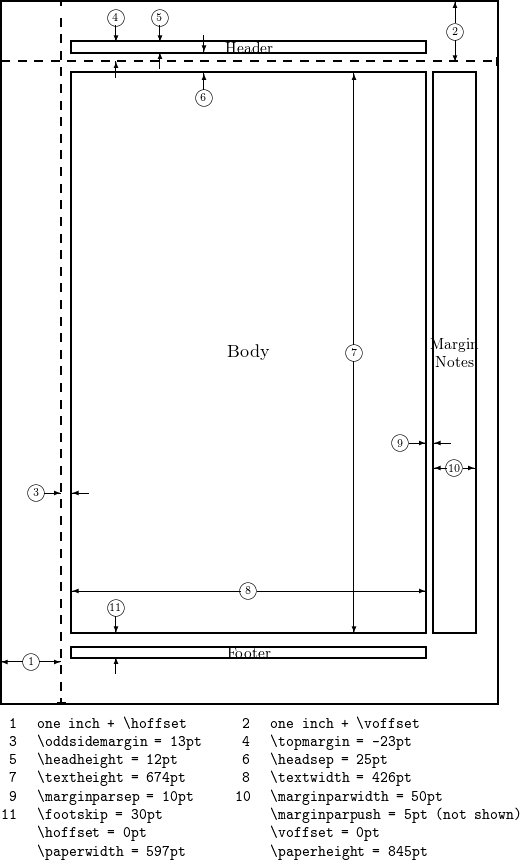
\includegraphics[width=0.85\linewidth]{Layout-dimensions.png}
\end{center}



\section{PoliceUtilisateur()}

\begin{lstlisting}
POLICE.taillefiche = '12pt'
POLICE.taillediapo = '20pt'
POLICE.tableau = '1.4'
POLICE.texte = 'Calibri'
POLICE.math = 'STIX Two Math'
POLICE.mathcal = 'Libertinus Math Regular'
POLICE.important = [[ \hl{#1} ]]
\end{lstlisting}

\begin{itemize}
  \item \texttt{taillefiche} : taille de police par défaut pour les documents au format \texttt{fiche}
  \item \texttt{taillediapo} : taille de police par défaut pour les documents au format \texttt{diapo}
  \item \texttt{tableau} : écartement naturel des lignes de tableaux (par défaut 140\%)
  \item \texttt{texte} : police par défaut pour le texte
  \item \texttt{math} : police par défaut pour le math mode
  \item \texttt{mathcal} : police par défaut pour les lettres calligraphiées en math mode
  \item \texttt{important} : style pour la commande \texttt{\textbackslash important} (par défaut, surligné)
\end{itemize}

Si les polices ne sont pas installées sur le système, la \texttt{classe-tex3R} procédera à une substitution par une police par défaut de \LaTeX. Attention, les polices mathématiques sont des polices spéciales. A voir : \href{https://tug.org/FontCatalogue/}{The \LaTeX Font Catalogue}


\section{CouleursUtilisateur()}

\subsection{if PRINT}

\begin{lstlisting}
COULEURS.ligne = 'black'
COULEURS.interligne = 'black!30'
COULEURS.section = 'black'
COULEURS.subsection = 'black!70'
COULEURS.subsubsection = 'black!40'
COULEURS.carreau = 'black!30'
COULEURS.surlignelignea = 'black!20'
COULEURS.surligneligneb = 'white'
COULEURS.boitecours = 'white'
COULEURS.background = 'white'

COULEURS.application = 'black'
COULEURS.definition = 'black'
COULEURS.convention = 'black'
COULEURS.exercice = 'black'
COULEURS.exemple = 'black'
COULEURS.methode = 'black'
COULEURS.preuve = 'black'
COULEURS.propriete = 'black'
COULEURS.remarque = 'black'
COULEURS.enonce = 'black'
COULEURS.correction = 'black'
COULEURS.surligne = 'black!5'
COULEURS.surlignevisible = 'black!10'

COULEURS.rouge = 'black'
COULEURS.bleu = 'black'
COULEURS.vert = 'black'
\end{lstlisting}

\subsection{else}

\begin{lstlisting}
COULEURS.ligne = 'SlateBlue'
COULEURS.interligne = 'LightSteelBlue'
COULEURS.section = 'black'
COULEURS.subsection = 'Red'
COULEURS.subsubsection = 'Green'
COULEURS.carreau = 'blue!25'
COULEURS.surlignelignea = 'blue!20'
COULEURS.surligneligneb = 'yellow!20'
COULEURS.boitecours = 'black!5'
COULEURS.background = 'white'

COULEURS.application = 'black'
COULEURS.definition = 'Green'
COULEURS.convention = 'black'
COULEURS.exercice = 'Blue'
COULEURS.exemple = 'Blue'
COULEURS.methode = 'black'
COULEURS.preuve = 'black'
COULEURS.propriete = 'Red'
COULEURS.remarque = 'black'
COULEURS.enonce = 'black'
COULEURS.correction = 'black'
COULEURS.surligne = 'yellow'
COULEURS.surlignevisible = 'black!10'

COULEURS.rouge = 'Red'
COULEURS.bleu = 'Blue'
COULEURS.vert = 'Green'
\end{lstlisting}

Toutes les couleurs sont définies dans la classe, il n'est pas possible d'en rajouter dans le \texttt{lua}. L'intérêt de ces couleurs, est de pouvoir changer leur valeur en fonction du paramètre \texttt{Impression}. Le nom des couleurs en \LaTeX{} est \texttt{couleur} + \texttt{variable} (par exemple : \texttt{couleursection} ou \texttt{couleurapplication})

\begin{itemize}
  \item \texttt{ligne} ; \texttt{interligne} : couleurs pour la commande \texttt{\textbackslash lignes\{seyes\}}
  \item \texttt{carreau} : couleur pour la commande \texttt{\textbackslash lignes\{carreau\}}
  \item \texttt{surlignea} ; \texttt{surligneb} : couleurs pour la commande \texttt{\textbackslash lignes\{surligne\}}
  \item \texttt{boitecours} : couleur de l'arrière plan des boîte de cours
  \item \texttt{background} : couleur de l'arrière plan des documents
  \item \texttt{surligne} : couleur de la commande \texttt{\textbackslash hl} utilisée par la commande \texttt{\textbackslash important}
  \item \texttt{rouge} ; \texttt{bleu} ; \texttt{vert} : couleurs du panel
\end{itemize}


\section{LogosUtilisateur()}

\begin{lstlisting}
LOGOS.activite = [[ \reflectbox{\faPencil*} ]]
LOGOS.basique = ''
LOGOS.bilan = [[ \faEdit[regular] ]]
LOGOS.corrige = [[ \faEdit[regular] ]]
LOGOS.cours = [[ \faBook ]]
LOGOS.DM = [[ \faHome ]]
LOGOS.DS = [[ \faFile*[regular] ]]
LOGOS.flash = [[ \faUserSecret ]]
LOGOS.interro = [[ \faFile*[regular] ]]
LOGOS.TD = [[ \faEdit[regular] ]]
\end{lstlisting}

Logos utilisés pour les titres, voir le package \href{https://mirrors.ircam.fr/pub/CTAN/fonts/fontawesome5/doc/fontawesome5.pdf}{fontawesome5}. Le logo est stocké dans \texttt{\textbackslash logoactif}, qui change en fonction du \texttt{Type}.

\section{StylesTitresUtilisateur()}

Les titres sont définis en trois temps :

\begin{enumerate}
  \item Le style global, commun à tous les titres (par défaut, un logo, et un contenu souligné sur toute la longueur)
  \item Le style particulier au \texttt{Type} du document (le nom du chapitre pour les fiches de TD ou faire apparaître NOM et Prénom pour les DS par exemple)
  \item Le mot clé à faire apparaître au bon endroit pour les titres partageant le même style (DM, interro ou DS par exemple)
\end{enumerate}


\subsection{Définition des styles}

\begin{lstlisting}
STYLESTITRES.espacement = '0.5cm'
STYLESTITRES.titre = [[ {\bfseries\LARGE\logoactif~\underLine{#1}\par} ]]
STYLESTITRES['sans'] = [[  ]]
STYLESTITRES['un'] = [[ \titre{#1\hfill\mdseries\large\contenuniveau} ]]
STYLESTITRES['deux'] = [[ \titre{#1~\mdseries|~\contenuchapitre\hfill\large\contenuniveau} ]]
STYLESTITRES['trois'] = [[ \titre{#1~\mdseries|~{\large\mdseries NOM :} \hfill {\large\mdseries Prénom :} \hfill \mdseries\large\contenuniveau} ]]
\end{lstlisting}

\begin{itemize}
  \item \texttt{espacement} : saut de ligne après le titre de début de page (à faire correspondre avec \texttt{PAGE.headerheadsep})
  \item \texttt{titre} : définit le style global à tous les titres, comme expliqué précedemment
\end{itemize}

Pour définir des styles particuliers de titre, les commandes \texttt{\textbackslash contenuniveau}, \texttt{\textbackslash contenuchapitre} (donnant le contenu des options \texttt{Niveau} et \texttt{Chapitre}) sont accessibles.

il est possible de créer d'autres styles de particuliers de titre dans le \texttt{lua} sur le même modèle, au besoin.

\subsection{if FORMAT == "fiche"}

\begin{lstlisting}
STYLESTITRES.activite = STYLESTITRES['un']
STYLESTITRES.basique = STYLESTITRES['sans']
STYLESTITRES.bilan = STYLESTITRES['un']
STYLESTITRES.corrige = STYLESTITRES['deux']
STYLESTITRES.cours = STYLESTITRES['deux']
STYLESTITRES.DM = STYLESTITRES['trois']
STYLESTITRES.DS = STYLESTITRES['trois']
STYLESTITRES.flash = STYLESTITRES['un']
STYLESTITRES.interro = STYLESTITRES['trois']
STYLESTITRES.TD = STYLESTITRES['deux']
\end{lstlisting}

\subsection{if FORMAT == "diapo"}

\begin{lstlisting}
STYLESTITRES.activite = STYLESTITRES['un']
STYLESTITRES.basique = STYLESTITRES['sans']
STYLESTITRES.bilan = STYLESTITRES['un']
STYLESTITRES.corrige = STYLESTITRES['deux']
STYLESTITRES.cours = STYLESTITRES['deux']
STYLESTITRES.DM = STYLESTITRES['trois']
STYLESTITRES.DS = STYLESTITRES['trois']
STYLESTITRES.flash = STYLESTITRES['un']
STYLESTITRES.interro = STYLESTITRES['trois']
STYLESTITRES.TD = STYLESTITRES['deux']
\end{lstlisting}

Il est possible de changer le style du titre selon que l'on est en format \texttt{fiche} ou en format \texttt{diapo}.

\section{TitresUtilisateur()}

\subsection{Formatage des titres}

\begin{lstlisting}
TITRES.format = [[ Activité ]]

TITRES.format = [[ ]]

TITRES.format = [[ Bilan ]]

TITRES.format = [[ Corrigé ]]

TITRES.format = [[ Chapitre~\thepart ]]

TITRES.format = [[ DM n°\stepcounter{compteurDM}\thecompteurDM ]]

TITRES.format = [[ DS n°\stepcounter{compteurDS}\thecompteurDS ]]

TITRES.format = [[ Questions Flash n°\stepcounter{compteurflash}\thecompteurflash ]]

TITRES.format = [[ Interrogation n°\stepcounter{compteurinterro}\thecompteurinterro ]]

TITRES.format = [[ TD ]]
\end{lstlisting}

\texttt{format} : permet de placer le mot clé dans l'emplacement du \#1 des \texttt{STYLETITRES['X']}

\subsection{Formatage de la TOC}

\begin{lstlisting}
TITRES.tocactivite = 'Activité'
TITRES.tocbasique = 'Sans titre'
TITRES.tocbilan = 'Bilan'
TITRES.toccorrige = 'Corrigé'
TITRES.toccours = 'Cours'
TITRES.tocDM = 'DM'
TITRES.tocDS = 'DS'
TITRES.tocflash = 'Flash'
TITRES.tocinterro = 'Interrogation'
TITRES.tocTD = 'TD'
\end{lstlisting}

Mot-clés apparaissant selon le \texttt{Type} de document choisi dans les signets du document.

\section{EnvironnementsUtilisateur()}

\subsection{Environnements de cours}

\begin{lstlisting}
ENVIRONNEMENTS.formatcours = [[
  \begin{tcolorbox}[
    colback=couleurboitecours, 
    colframe=couleurbackground, 
    boxrule=0pt, 
    left=0.5em, 
    top=0pt, 
    bottom=0pt, 
    right=0pt, 
    enhanced, 
    shield externalize=true, 
    borderline west={4pt}{0pt}{#2}
    ]
    \textcolor{#2}{\large\underLine{#1} :}\par
    \medskip 
    \BODY 
  \end{tcolorbox}
  ]]
\end{lstlisting}

\subsection{Environnement enonce}

\begin{lstlisting}
ENVIRONNEMENTS.enonce = [[
  \iftheme
    \hfill{\itshape\footnotesize\contenutheme}\par\vspace{0.2em}{\color{couleurenonce}\hrule height 2pt}\par
  \fi
  \colorbox{couleurenonce}{\textcolor{white}{
    {
    \Large\textbf{\thecompteurexercice}}
    \ifdifficulte{~\raisebox{0.2em}{\scriptsize\contenudifficulte}}\fi
    }
  }
  \ifcompetence\hspace{0.3em}\textcolor{couleurenonce}{\underLine{\large\raisebox{0.1em}{\contenucompetence}}}\fi\ifbareme\hfill {\bfseries/\contenubareme~points}\fi\par
    \medskip
    \BODY
    \ifsource\par
      \vspace{0.2em}{\color{couleurenonce}\hrule height 2pt}\par\vspace{0.2em}\hfill{\itshape\footnotesize\contenusource}
    \fi
]]
\end{lstlisting}

\subsection{Environnement correction}

\begin{lstlisting}
ENVIRONNEMENTS.correction = [[
  \colorbox{couleurcorrection}{\textcolor{white}{
    \normalfont\Large\textbf{\thecompteurexercice} | Correction}
  }\par
  \medskip
  \BODY
]]
\end{lstlisting}

\subsection{Formatage de la TOC}

\begin{lstlisting}
ENVIRONNEMENTS.tocexercice = 'Exercice'
ENVIRONNEMENTS.tocenonce = 'Énoncé'
ENVIRONNEMENTS.toccorrection = 'Correction'
\end{lstlisting}

\section{mesParametres(str)}

\begin{lstlisting}
function mesParametres(str)

  if str == 'activite' or str == 'Activite' then
    Type = 'activite'
    Impression = true
    Competence = true
    Enonce = true
    Stretch = true
  elseif str == 'basique' or str == 'Basique' then

  elseif str == 'bilan' or str == 'Bilan' then
    Type = 'bilan'
    Impression = true
    Competence = true
    Enonce = true
    Stretch = true
  elseif str == 'corrige' or str == 'Corrige' then

  elseif str == 'cours' or str == 'Cours' then
    Type = 'cours'
    Enonce = true
    Correction = true
    Stretch = false
  elseif str == 'DM' then
    Type = 'DM'
    Impression = true
    Competence = true
    Enonce = true
    Stretch = true
  elseif str == 'DS' then
    Type = 'DS'
    Impression = true
    Competence = true
    Enonce = true
    Stretch = true
    Bareme = true
  elseif str == 'flash' or str == 'Flash' then

  elseif str == 'interro' or str == 'Interro' then
    Type = 'interro'
    Impression = true
    Competence = true
    Enonce = true
    Stretch = true
    Bareme = true
  elseif str == 'TD' then
    Type = 'TD'
    Header = true
    Impression = true
    Competence = true
    Enonce = true
    Stretch = true
  end
end
\end{lstlisting}

\section{NiveauUtilisateur(arg)}

\begin{lstlisting}
function NiveauUtilisateur(arg)
  local str = nil
  if arg == '6' then
    str = '6$^\\text{ème}$'
  elseif arg == '5' then
    str = '5$^\\text{ème}$'
  elseif arg == '4' then
    str = '4$^\\text{ème}$'
  elseif arg == '3' then
    str = '3$^\\text{ème}$'
  end
  NiveauDocument(str) 
end
\end{lstlisting}

\end{document}